\chapter{Backgrounds}
\label{sec:background}

In this chapter, we briefly review related backgrounds.

\section{E-graphs and e-matching}

\paragraph{Terms.}
Let $\Sigma$ be a set of function symbols with associated arities. 
A function symbol is called a \textit{constant} if it has a zero arity. 
Let $V$ be the set of variables. We define $T(\Sigma, V)$ to be the set of terms constructed using function symbols from $\Sigma$ and variables from $V$. 
More formally, $T(\Sigma, V)$ is the smallest set that (1) all variables and constants are in $T(\Sigma,V)$ and (2) $t_1,\dots,t_k\in T(\Sigma,V)$ implies $f(t_1,\dots,t_k)\in T(\Sigma,V)$, where $f\in \Sigma$ has arity $k$. 
A \textit{ground term} is a term in $T(\Sigma,V)$ that contains no variables. A non-ground term is also called a \textit{pattern}. We call a term of the form $f(t_1,\ldots,t_k)$ an $f$-application term.

\paragraph{Congruence relation.}
An \textit{equivalence relation} $\equiv_\Sigma$ is a binary relation over $T(\Sigma,\emptyset)$ that is reflexive, symmetric, and transitive. A \textit{congruence relation} $\cong_\Sigma$ is an equivalence relation satisfying that if $t_i\cong t'_i$ for all $i=1,\dots,n$ hold, $f(t_1,\dots,t_n)\cong f(t'_1,\dots,t'_n)$ holds as well, where $f$ is a $n$-ary function symbol. We wrote $\cong$ when $\Sigma$ is clear from the context.


\paragraph{\Egraph.}
Intuitively, an \egraph $E$ is a set of \eclasses $\{c_1, \ldots, c_k\}$, where each \eclass $c$ is a set of \enodes $\{n_1,\ldots,n_k\}$. Each \enode consists of a function symbol $f$ and a list of children \eclasses. 
Similar to patterns, we call an \enode of the form $f(c_1, \ldots c_n)$ an $f$-application \enode.
More formally, we define an \egraph $E$ to be an tuple $(\Sigma,N,C,\textit{symbol}, \textit{lookup}, \textit{child})$ where 
\begin{itemize}
    \item $\Sigma$ is a set of function symbols with associated arities,
    \item $N$ is the set of \enodes,
    \item $C$ is the set of \eclasses,
    \item \textit{symbol} is a function that maps each \enode in $N$ to a function symbol in $\Sigma$,
    \item \textit{lookup} is a function that maps every \enode in $N$ to the \eclass in $C$ that contains it, and
    \item \textit{child} is a function that maps an $\enode$ to a list of \eclass that are the children of this \enode.
\end{itemize}
For convenience, we use $n.\sym$, $n.\textit{id}$, and $n.\child_i$ to denote $\textit{symbol}\,(n)$, $\textit{lookup}\,(n)$, and the $i$th element of $\child(n)$.

An \egraph $E$ efficiently represents sets of ground terms in a congruence relation. 
An \egraph is said to \textit{represent} a ground term $t$ if its \eclasses represent it.
An \eclass $c$ represents a ground term if $c$ contains an \enode $a$ that represents it. 
An \enode $f(c_1,\dots,c_k)$ represents a ground term $f(t_1,\dots,t_k)$ if they have the same function symbol $f$ and each e-class $c_i$ represents term $t_i$.
Terms represented by an \eclass are equivalent to each other.
Consequently, an \egraph forms a congruence relation.
Consider \autoref{fig:egraph} for example. $g(f(c,c))$, $f(c, g(b))$, and $f(a, g(a))$ are three ground terms represented by \eclass $c_1$ in this \egraph. Therefore, they are congruent with each other by definition.

\begin{figure}[!t]
    \hspace{-2em}
  \begin{tabular}[b]{cc}
    \begin{subfigure}[b]{0.45\linewidth}
        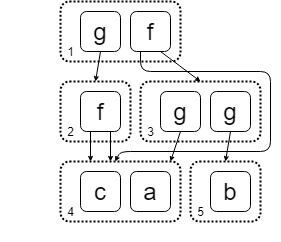
\includegraphics[width=\linewidth]{figures/egraph.png}
      \caption{}
      \label{fig:egraph}
    \end{subfigure}
    \begin{tabular}[b]{c}
      \begin{subfigure}[t]{0.45\columnwidth}
      \centering
        \begin{tabular}{|ccc|}
            \hline
            eclass-id & $\text{child}_1$ & $\text{child}_2$ \\
            \hline
            1         & 4        & 3        \\
            2         & 4        & 4       \\
            \hline
        \end{tabular}
        \caption{}
        \label{fig:repr-f}
      \end{subfigure}\\
      \begin{subfigure}[b]{0.5\columnwidth}
      \centering  
        \begin{tabular}{|cc|}
            \hline
            eclass-id & $\text{child}_1$ \\
            \hline
            1         & 2         \\
            3         & 4         \\
            3         & 5         \\
            \hline
        \end{tabular}
        \caption{}
        \label{fig:repr-g}
      \end{subfigure}
    \end{tabular}
  \end{tabular}
  \caption{(a) an e-graph over $T(\Sigma, \emptyset)$ and  $\cong_\Sigma$ where $\Sigma=\{f,g,a,b,c\}$ and $a,b,c$ are nullary functions. Each solid box denotes an e-node and each dashed box denotes an e-class. Every term represented by an e-class is mutually equivalent. For example, $a\cong_\Sigma c$, $g(a)\cong_\Sigma g(b)$, and $f(a, g(a)) \cong_\Sigma g(f(a, a))$. The labels of e-classes are at bottom left.\quad (b) relation representing $f$. \quad(c) relation representing $g$.}
\end{figure}

\paragraph{\Ematching.}
\Ematching is the task of finding \ematching substitutions that instantiate patterns to set of terms represented in the \egraph. 
An \textit{\ematching substitution} $\sigma$ is a function that maps every variable in a pattern to e-classes.
For convenience, we use $\sigma(p)$ to denote the set of terms obtained by replacing every occurrence of variable $v_i$ in $p$ with terms in $\sigma(v_i)$.
Formally, given an e-graph $E$ and a pattern $p$,  \ematching finds the set of all possible pairs $(\sigma, r)$ such that every term in $\sigma(p)$ is represented in the e-class $r$.
Terms in $\sigma(p)$ are said to be matched by pattern~$p$. $r$ is said to be the root of matched terms.
For instance, pattern $f(\alpha, g(\alpha))$
 matches four terms in e-class $c_1$: $f(a, g(a))$, $f(a, g(c))$, $f(c,g(c))$, and $f(c, g(a))$; 
 all of which are witnessed by the substitution $\{\alpha \mapsto c_4\}$.

Existing approaches to e-matching rely on backtracking \citep{efficient-ematching,simplify,egg}. 
For example, \citet{efficient-ematching} proposed a backtracking-based e-matching algorithm that is used by \textsc{Z3} \citep{Z3} and \egg \citep{egg}, two state-of-the-art e-graph implementations. 
To match the pattern $f(\alpha, g(\alpha))$ on the e-graph in Figure \ref{fig:egraph}, their algorithm does a depth-first search over the e-graph:
% Conceptually, it recursively searches for the pattern $f(\alpha, g(\beta))$ and filters out substitutions that map $\alpha$ and $\beta$ to different e-classes.
it searches for all $f$-application e-nodes $n_f$, adds $\alpha\mapsto n_f.\textit{child}_1$ to substitution $\sigma$, iterates through all $g$-application e-nodes $n_g$ in e-class $n_f.\textit{child}_2$, and only yield $\sigma$ if $n_g.\textit{child}_1=\sigma(\alpha)$.
In general, this procedure runs in time that is quadratic of the \egraph size.
In a large e-graph, there may be thousands of pairs of $n_f$ and $n_g$ where $n_g$ is in e-class $n_f.\textit{child}_2$, but only a few satisfy the constraint $n_f.\textit{child}_1=n_g.\textit{child}_1$. Therefore, backtracking-based \ematching enumerates an unnecessarily large pool of candidates.
Even worse, complex query patterns may involve many variables that occur at several places, which makes na\"ive backtracking enumerates an excessive number of terms and therefore extremely slow. 
This inefficiency is due to the fact that na\"ive backtracking does not use the equality constraints to prune the search space \textit{globally}. 
This is in contrast to our approach, which exploits the equality constraints during query planning for greater performance and guarantees worst-case optimality with respect to the output size.
  

\section{Conjunctive queries}

\paragraph{Relational schema.}
A relational schema $S_D$ over domain $D$ is a set of relation symbols with associated arities. An atom under a schema $S_D$ is an expression $R(t_1,\ldots,t_k)$, where $k$ is the arity of $R$ in $S_D$ and $t_i$ is an element in $D$. An instance of $S_D$ is a set of atoms over $S_D$. 

\paragraph{Conjunctive queries.}
A conjunctive query over schema $S_D$ and a set of variables $V$ is a formula of the form
\[
    \textit{ans}(x_1,\ldots x_k)\textit{ :- } R_1(v_{1,1},\ldots,v_{1,k_1}),\ldots, R_n(v_{n,1},\ldots,v_{n,k_n}),
\]
where $n\geq 0$, $R_1\ldots R_n$ are relation names in $S_D$ with arities $k_1,\ldots k_n$, \textit{ans} is the name of the resulting relation not in $S_D$, $v_{i,j}$ are variables in $V$\footnote{Some definitions of conjunctive queries allow both variables and constants, but we only allow variables in conjunctive queries for simplicity.}, and $x_1,\ldots x_k$ are variables occurring in $v_{i,j}$. We call such $R_i(v_{i,1},\ldots,v_{i,k_1})$ an atom of the conjunctive query.

\paragraph{Semantics of conjunctive queries.} 
Similar to \ematching substitutions, we define a conjunctive query substitution as a function that maps every variable occurring in $v_{i,j}$ to elements in $D$. The semantics of conjunctive queries is defined as follows: Let $q$ be a conjunctive query, $I$ be an instance of $S_D$, conjunctive queries yield the set of all $\textit{ans}(\sigma(x_1),\ldots,\sigma(x_k))$ where $\sigma$ is a substitution satisfying that $R_i(\sigma(t_1),\ldots \sigma(t_k))$ are atoms in $I$ for $i=1,\ldots,n$. We denote the result set as $q(I)$.

We make the observation that the definition of conjunctive query and \ematching
are definitionally similar to each other: both are defined as finding
substitutions whose instantiations are present in a (relational or graph)
database. In fact, the \ematching problem can be viewed as a ``nested''
conjunctive queries on a database where the atoms are nested. Therefore, it is
tempting to reduce the \ematching problem to a conjunctive query over the
relational database, thereby benefiting from well-studied techniques from the
database community, including join algorithms, query optimization, and query
evaluations.

\section[The AGM bound]{The AGM bound and Generic Join \footnote{This section is inspired by Remy Wang's \href{https://gitlab.com/remywang/blog/-/blob/master/posts/wcoj.md}{introduction to generic join algorithms}.}}

\algrenewcomment[1]{\(\triangleright\) #1}
\algnewcommand{\LineComment}[1]{\State \(\triangleright\) {\it #1}}
\paragraph{The AGM Bound}
\begin{figure}
  \centering
\begin{algorithmic}[1]
\Procedure{SolveTriangleQuery}{$R,S,T$}
\State $A := R(x,y).x \cap T(z,x).x$\;
  \LineComment{Compute $Q(\alpha,y,z) \textit{ :- } R(\alpha,y),S(y,z),T(z,\alpha)$}
  \For{$\alpha\in A$} 
  \State $B := R(\alpha,y).y \cap S(y,z).y$\;
    \LineComment{Compute $Q(\alpha,\beta,z) \textit{ :- } R(\alpha,\beta),S(\beta,z),T(z,\alpha)$}
    \For{$\beta \in B$}
        \State $C := S(\beta,z).z \cap T(z,\alpha).z$\;
        \LineComment{Yield join results $Q(\alpha, \beta, \gamma)$}
        \For{$\gamma \in C$}
        \State {\bf output } $Q(\alpha,\beta,\gamma)$
        \EndFor
    \EndFor
  \EndFor
\EndProcedure
  \caption{Generic join algorithm for the triangle query $Q(x,y,z) \textit{ :- } R(x,y),S(y,z),T(z,x)$, with ordering $[x, y, z]$.}\label{alg:gj}
\end{algorithmic}
\end{figure}

Given a database and a conjunctive query, the AGM bound \cite{agm} is a bound on how large the query output could be. A simple bound just multiplies the cardinally of each relation, which is the size of the Cartesian product of all relations. 
For example, for triangle query $ Q(x,y,z) \textit{ :- } R(x,y), S(y,z), T(x,z)$, this  bound computes to $|Q| \leq |R| \times |S| \times |T|$. 
If $|R|=|S|=|T|=N$, then $|Q| \leq N^3$.
However, we can do better: we observe that $Q$ contains fewer atoms than the query
$ Q’(x,y,z)\textit{ :- } R(x,y), S(y,z),$ as $Q$ is further filtered by joining with $T$. Therefore, we know $|Q| \leq |R| \times |S| = N^2$. 
In fact, the theoretical bound of conjunctive query output size is given as the AGM bound \citep{agm}, which is $N^{3/2}$ in this case.

The AGM bound proposes a question: is there an algorithm that always achieves the performance described by the AGM bound? In particular, \textit{cyclic queries} is a kind of conjunctive queries whose query hypergraph contains cycles, such as the triangle query $Q$ above, and they are known to make traditional join plans (e.g., join plans using two-way joins like hash joins or merge joins) suboptimal. Most of real-world database systems therefore have bad performance on cyclic queries.

\paragraph{Generic join.} Fortunately, theoretical progress has been made in the database theory community to achieve optimal performance on conjunctive queries and on cyclic queries in particualr. In particular, the generic join algorithm for conjunctive query is developed that runs in time linear to the worst-case output size with a log factor \citep{wcoj}. 
The generic join algorithm has great performance in practice when the query is cyclic, and is competitive to traditional join algorithms in other cases.
Given a conjunctive query and a relational database, generic join is parameterized over a ordering of the set of variables in the query, say $[x,y,z]$ for the query above. The ordering does not matter for the optimality guarantee, but may impact practical performance greatly. 
Given an ordering,
we assume the input relations are stored in tries sorted by the ordering.
That is, given the ordering $[x,y,z]$,
$R(x,y)$ is sorted by $x$ and then $y$,
and the first-level trie nodes are the $x$'s.
% Even more concretely,
% Figrue~\ref{fig:trie} illustrates the trie
% representing $R=\{(3, 4), (2, 1), (2, 5)\}$.
We can very efficiently intersect (join) relations on their
first (according to the variable ordering) variable given such tries.
Algorithm~\ref{alg:gj} shows the generic join algorithm for computing $Q$.
Note that selection, e.g. $R(a, y)$ is very fast with the built tries.
$A \cap B$ can also be done in $\tilde{O}(\min(|A|, |B|))$ time
($\tilde{O}$ means $O$ with a log factor).
For general queries we may have to intersect more than two relations,
in which case the intersection should be performed in
$\tilde{O}(\min_i|A_i|)$ time (using the merge in merge-sort).
